\documentclass[11pt]{article}
\usepackage[utf8]{inputenc}
\usepackage[T1]{fontenc}

\usepackage{amsfonts,amsmath,amssymb,graphicx}
\usepackage[portuguese]{babel}
\usepackage{txfonts}
\usepackage[left=2cm,right=3cm,top=3cm,bottom=2cm]{geometry}
\usepackage[dvipsnames]{xcolor}
\usepackage[hidelinks]{hyperref}



\hypersetup{
colorlinks = true,
urlcolor= Blue,
}


%\usepackage[]{}
%\setlength{\parindent}{12pt}
%\setlength{\parskip}{12pt}

\begin{document}
\begin{center}
\huge \sc Curriculum Vitae\\
\Large \sc Junior Rodrigues Ribeiro
\end{center}

\begin{flushright}
\fbox{
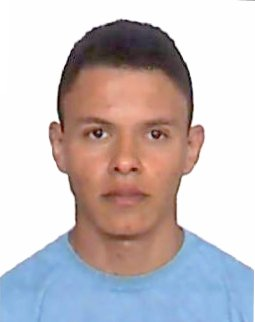
\includegraphics[width=3cm]{Avatar}
}
\end{flushright}
\vspace*{-4.4cm}

\section{Dados pessoais\dotfill  \hspace{3.4cm}\ }
\begin{description}
\item[Nome:] Junior Rodrigues Ribeiro.
\item[Celular/WhatsApp:] (16) 98253-4027.
\item[E-mail:] \href{mailto:j5r@outlook.com}{\nolinkurl{j5r@outlook.com}}, meu \href{http://lattes.cnpq.br/3866983332299702}{\texttt{CV Lattes}}\footnote{Para possibilitar clicar e seguir os links em azul, faça download deste arquivo.}.\item[Endereço:] Pq. Arnold Schmidt, São Carlos -- SP.
\item[Escolaridade:] Graduado em Matemática Licenciatura Plena pela UEMS, 2015,\\
\phantom{Escolarid} Mestre em Ciências (Ciências Matemáticas e Computação) pelo ICMC/USP, 2019.\\
\phantom{Escolarid} Doutorando em Ciências (Ciências Matemáticas e Computação) pelo ICMC/USP, 2022.
\end{description}

\section{Mais sobre mim \dotfill}
Comecei minha graduação em Matemática Licenciatura, foi minha primeira escolha de curso, pois amo compartilhar conhecimento. Resolvi ir além e preparar-me para docência a nível superior, e portanto segui com o mestrado. No momento acabo de iniciar o doutorado no programa de Matemática Computacional do ICMC.  Não tenho grande experiência em ministrar aulas, pois sempre segui estudando ininterruptamente (graduação, mestrado e agora doutorado).


Também amo música, aprendi teoria em aulas musicais na igreja. Já participei da Orquestra Jovem da UEMS na minha época de graduação, participando como violinista em uma época e como flautista doce em outro período. Fui medalhista de bronze da 7ª OBMEP (2011), motivo que me inclinou à área de Matemática em 2012, em vez de Música.

Aprendi uma porção de coisas sobre programação (precisei aprender para desenvolver programas para resolverem os problemas matemáticos do mestrado). No momento continuo estudando alguns materiais sobre tecnologia, pois acabei fascinado pela área e no entanto não tenho formação em computação, o que me impulsiona a aprender por conta própria coisas de meu interesse.

Objetivo conseguir uma oportunidade para trabalhar, compartilhar um pouco do conhecimento adquirido, mas que me permita continuar com meus estudos e pesquisas. Quem sabe eu consiga motivar alunos a seguirem os mesmos passos em busca de conhecimento. 
 

 
\section{Conhecimentos em programação e outros \dotfill}
\begin{itemize}
\item Idiomas: \\Espanhol --- Básico/Intermediário;\\ Inglês --- Básico/Intermediário;

\item Escritório: Tenho conhecimentos em Microsoft Word, Excel, Power Point e Outlook e suas versões do pacote Libre Office; boas habilidades de escrita e correção ortográfica; conhecimentos de LaTeX.

\item Ambientes: Windows e Linux (uso a versão Mint);

\item Programação:
\begin{itemize}
\item Formato: Estruturada; Orientada a Objeto (POO);
\item Científica: Matlab; C/C++ (nível básico); Python Numpy, Matplotlib;
\item Web: básico de HTML/CSS; Python BeautifulSoup, Selenium;
\item Dados: Python Pandas, Sqlite3, Shelve, OpenPyXL;
\item Desktop: Python OS, Multiprocessing, Threading;
\item GUI: Python Tkinter;
\item Outros: \href{https://github.com/j5r}{\texttt{GitHub}}\footnote{Para possibilitar clicar e seguir os links em azul, faça download deste arquivo.}; Markdown;
\end{itemize}

\item Científico: Já estudei disciplinas de otimização: Programação Linear, Inteira, Não-Linear, Dinâmica. Meu trabalho de mestrado foi em Sistemas Dinâmicos/Teoria de Controle, não em Otimização/Pesquisa Operacional (PO).

\end{itemize}


\section{Experiências anteriores \dotfill}
\begin{enumerate}
\item ESTAGIÁRIO, REFORÇO DE MATEMÁTICA, \textit{EE Pastor Daniel Berg. Dourados -- MS.} Duração de 8 meses, de abril a novembro de 2012. Atividade: ministrar reforço de matemática nas turmas de sexto a nono anos do ensino fundamental (bolsa de extensão universitária da UEMS).

\item ESTAGIÁRIO, COORDENAÇÃO PEDAGÓGICA. {\it FATEC SENAI Dourados -- MS}. Duração de 2 anos, de agosto de 2013 a agosto de 2015. Atividades: criação e geração de relatórios de desempenho e presença dos alunos para envio às empresas contratantes; agendamento de aulas no sistema integrado; atendimento e acompanhamento de questões diversas relacionadas a alunos; {\it check list} de diários dos professores para arquivamento. 


\item OUTRAS EXPERIÊNCIAS, sem finalidade acadêmica:
\begin{enumerate}
\item  Auxiliar de Garçom (finais de semana), 1 mês (novembro de 2012), pizzaria Mordomos do Rei, Dourados--MS;
\item Auxiliar de Escritório (CLT), 7 meses (dezembro de 2012 a junho de 2013), Toldos Líder, Dourados -- MS;
\item  Serviços Gerais (temporário), 2 meses (junho a julho de 2016), JPP Restaurante Prato Rápido Mineiro, São Carlos -- SP.
\end{enumerate}
\end{enumerate}

\end{document}
